\title{Recitation 9} 
\author{AVL Trees and Median finding in linear time.}
\documentclass{article}


\usepackage[utf8]{inputenc}
\usepackage[a4paper, total={6in, 9in}]{geometry}
\usepackage{braket}
\usepackage{xcolor}
\usepackage{amsmath}
\usepackage{amsfonts}
\usepackage{tikz}
\usepackage{svg}
\usepackage{graphicx}
\usepackage{media9}
\usepackage{float}
\usetikzlibrary{calc}
\usepackage{array}
\usepackage[ruled,vlined,linesnumbered]{algorithm2e}

\usepackage[
backend=biber,
style=alphabetic,
sorting=ynt
]{biblatex}



\newcommand{\commentt}[1]{\textcolor{blue}{ \textbf{[COMMENT]} #1}}
\newcommand{\ctt}[1]{\commentt{#1}}
\newcommand{\prb}[1]{ \mathbf{Pr} \left[ {#1} \right]}
\newcommand{\onotation}[1]{\(\mathcal{O} \left( {#1}  \right) \)}
\newcommand{\ona}[1]{\onotation{#1}}
\newcommand{\nvar}[2]{ \( #1_{1}, #1_{2} ... #1_{#2}  \) }
%\newenvironment{proof}[0]{\paragraph{Proof.}}{}
%\newenvironment{remark}[0]{\textit{remark}}{}
\newenvironment{cor}[0]{\paragraph{Corollary.}}{}
\newenvironment{example}[0]{\paragraph{Example.}}{}
%\newenvironment{thm}[0]{\paragraph{Theorem.}}{}
\newtheorem{prop}{Proposition}
\newtheorem{ex}{Exercise}
\newtheorem{sol}{Solution}
\newtheorem{theorem}{Theorem} 		
\newtheorem{thm}{Theorem}[section]
\newtheorem{conj}[thm]{Conjecture} 	
\newtheorem{lemma}[thm]{Lemma}
\newtheorem{corollary}[thm]{Corollary} 
\newtheorem{claim}[thm]{Claim}
\newtheorem{proposition}[thm]{Proposition}
\newtheorem{definition}{Definition} 
\newtheorem{remark}{Remark}
 


% \addbibresource{sample.bib} %Import the bibliography file
\begin{document}    
\maketitle

\begin{abstract}
     In the last week, we have seen that most of the operations over \textbf{BST} required cost in the order of the tree height. The \textbf{AVL} data structure addresses that problem by enforcing the tree's height to be logarithmic in its size.
\end{abstract}

\paragraph{Recitation Goals:}
\begin{enumerate}
    \item Review the Avl Trees. 
    \item Present a linear time algorithm for finding the median of \(n\) elements. And on the way, demonstrate another correction proof. 
\end{enumerate}


\section{Avl Trees Review.}
The conceptual idea which sharing. 

\begin{tabular}{ m{5cm} m{11cm}  }
     Recall that in the last recitation, we saw how probability could help us analyze algorithms that have assumptions over the distribution of the inputs & \resizebox{220}{150}{
        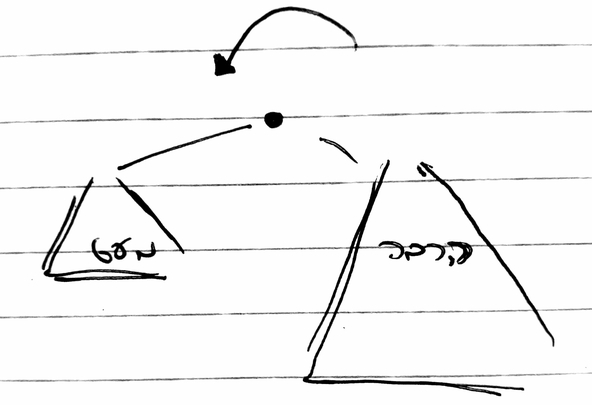
\includegraphics{tex/lectures-TA/dast_4.jpg}
    }
\end{tabular}


     \resizebox{16cm}{5cm}{
        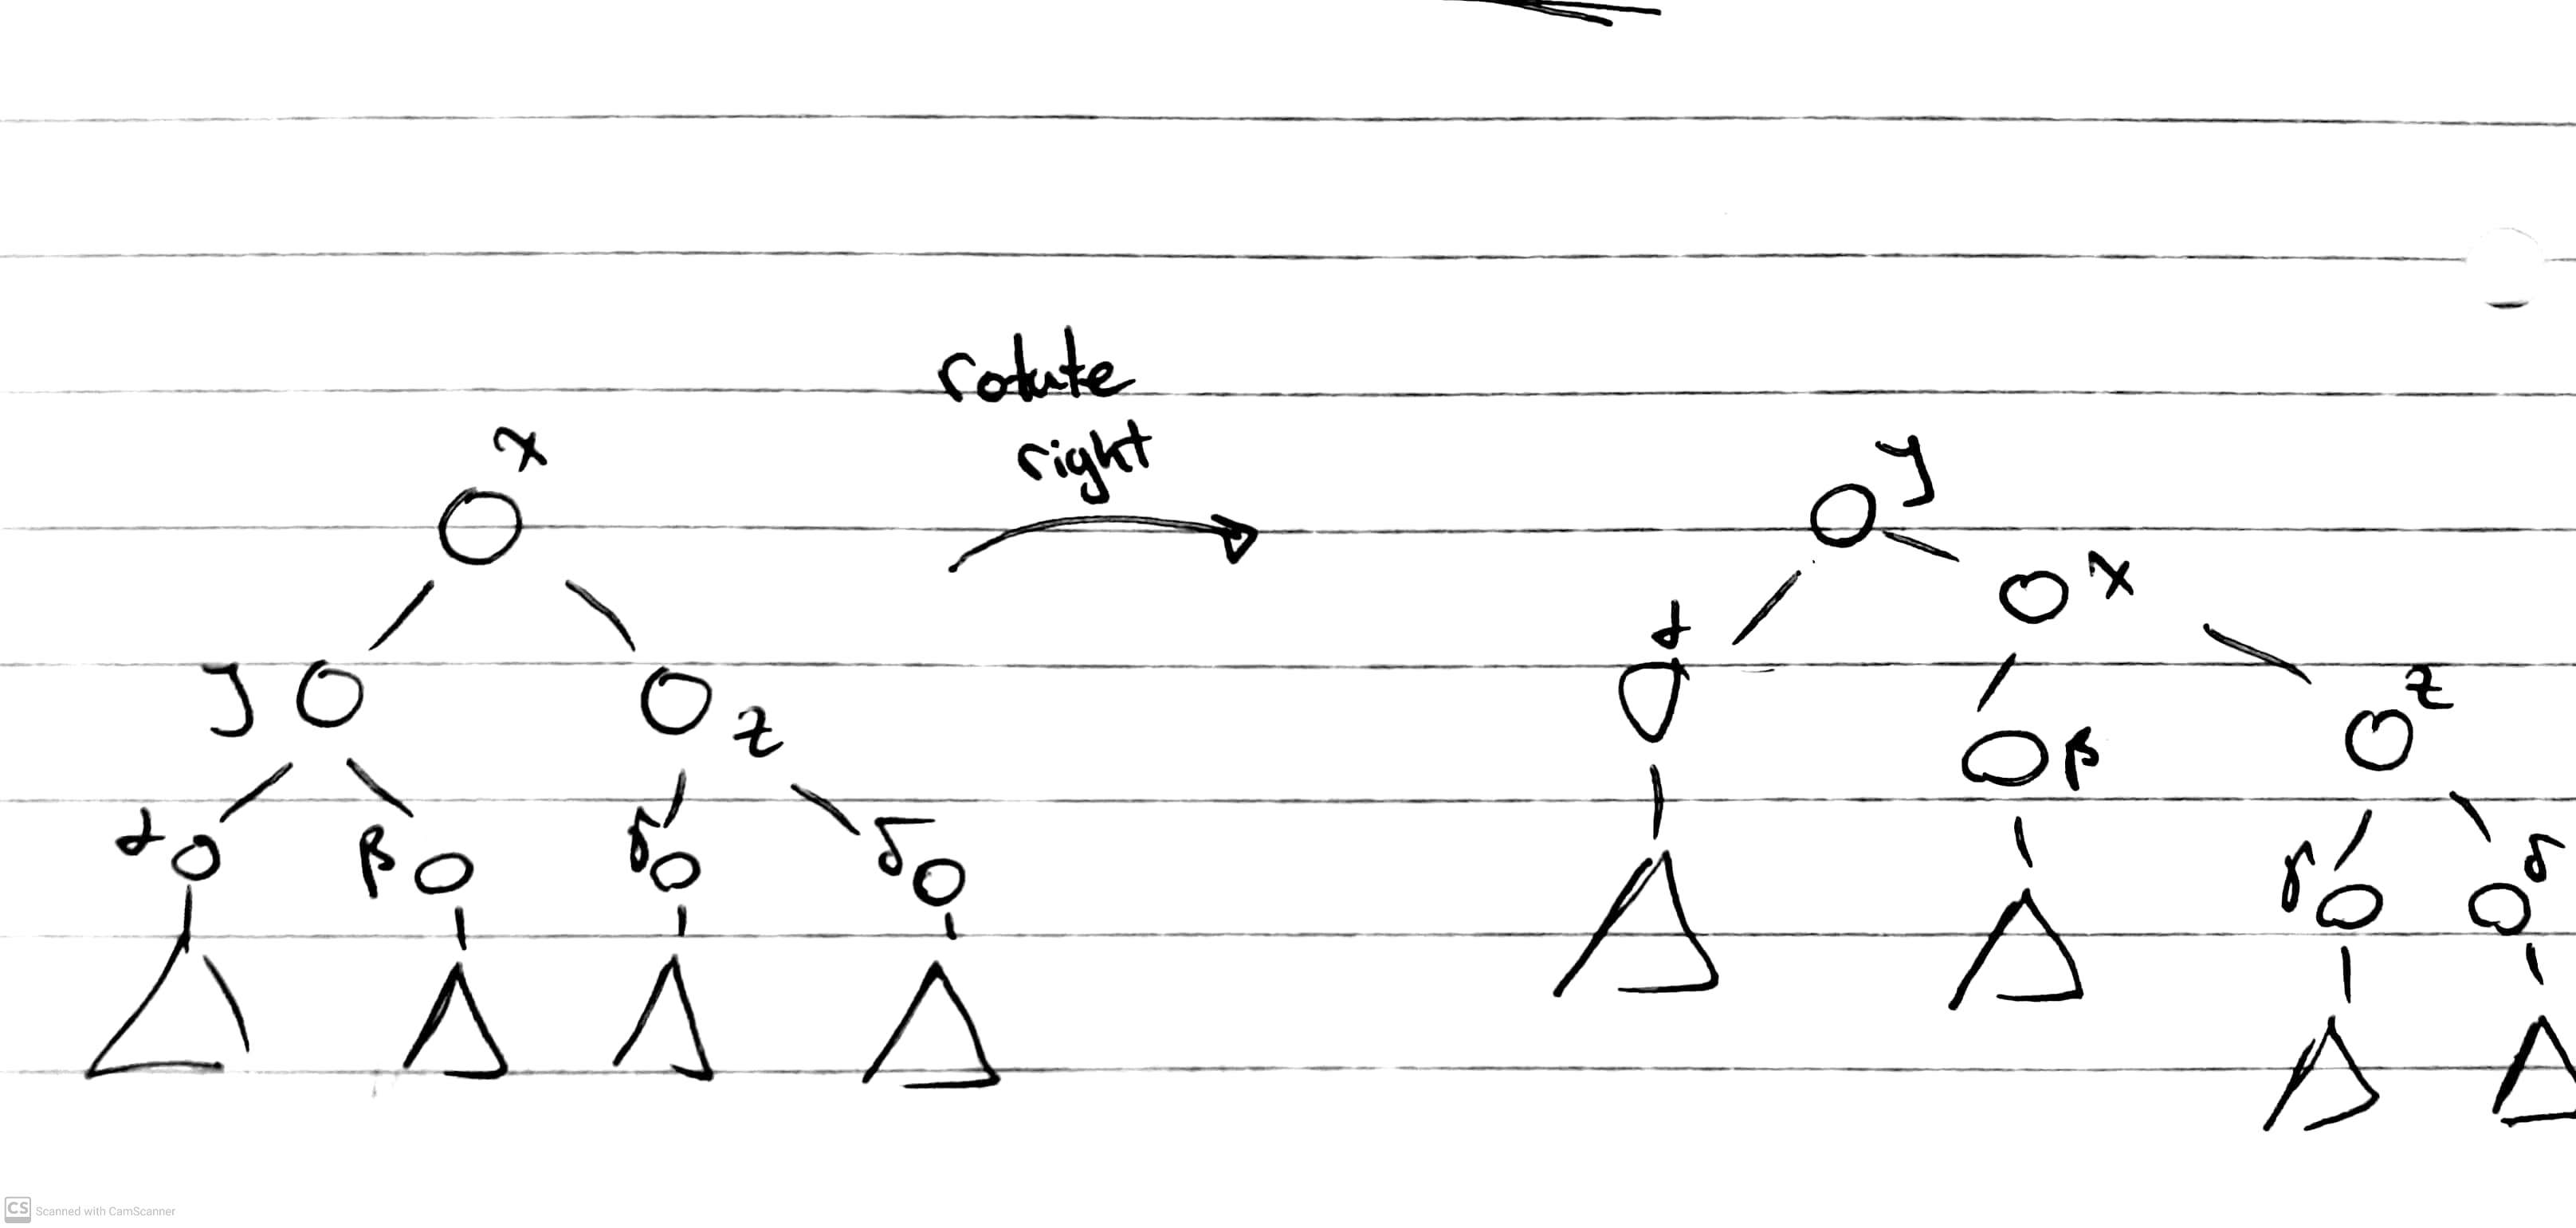
\includegraphics{tex/lectures-TA/dast_2.jpg}
    }

\begin{tabular}{ m{5cm} m{11cm}  }
     Recall that in the last recitation, we saw how probability could help us analyze algorithms that have assumptions over the distribution of the inputs & \resizebox{220}{150}{
        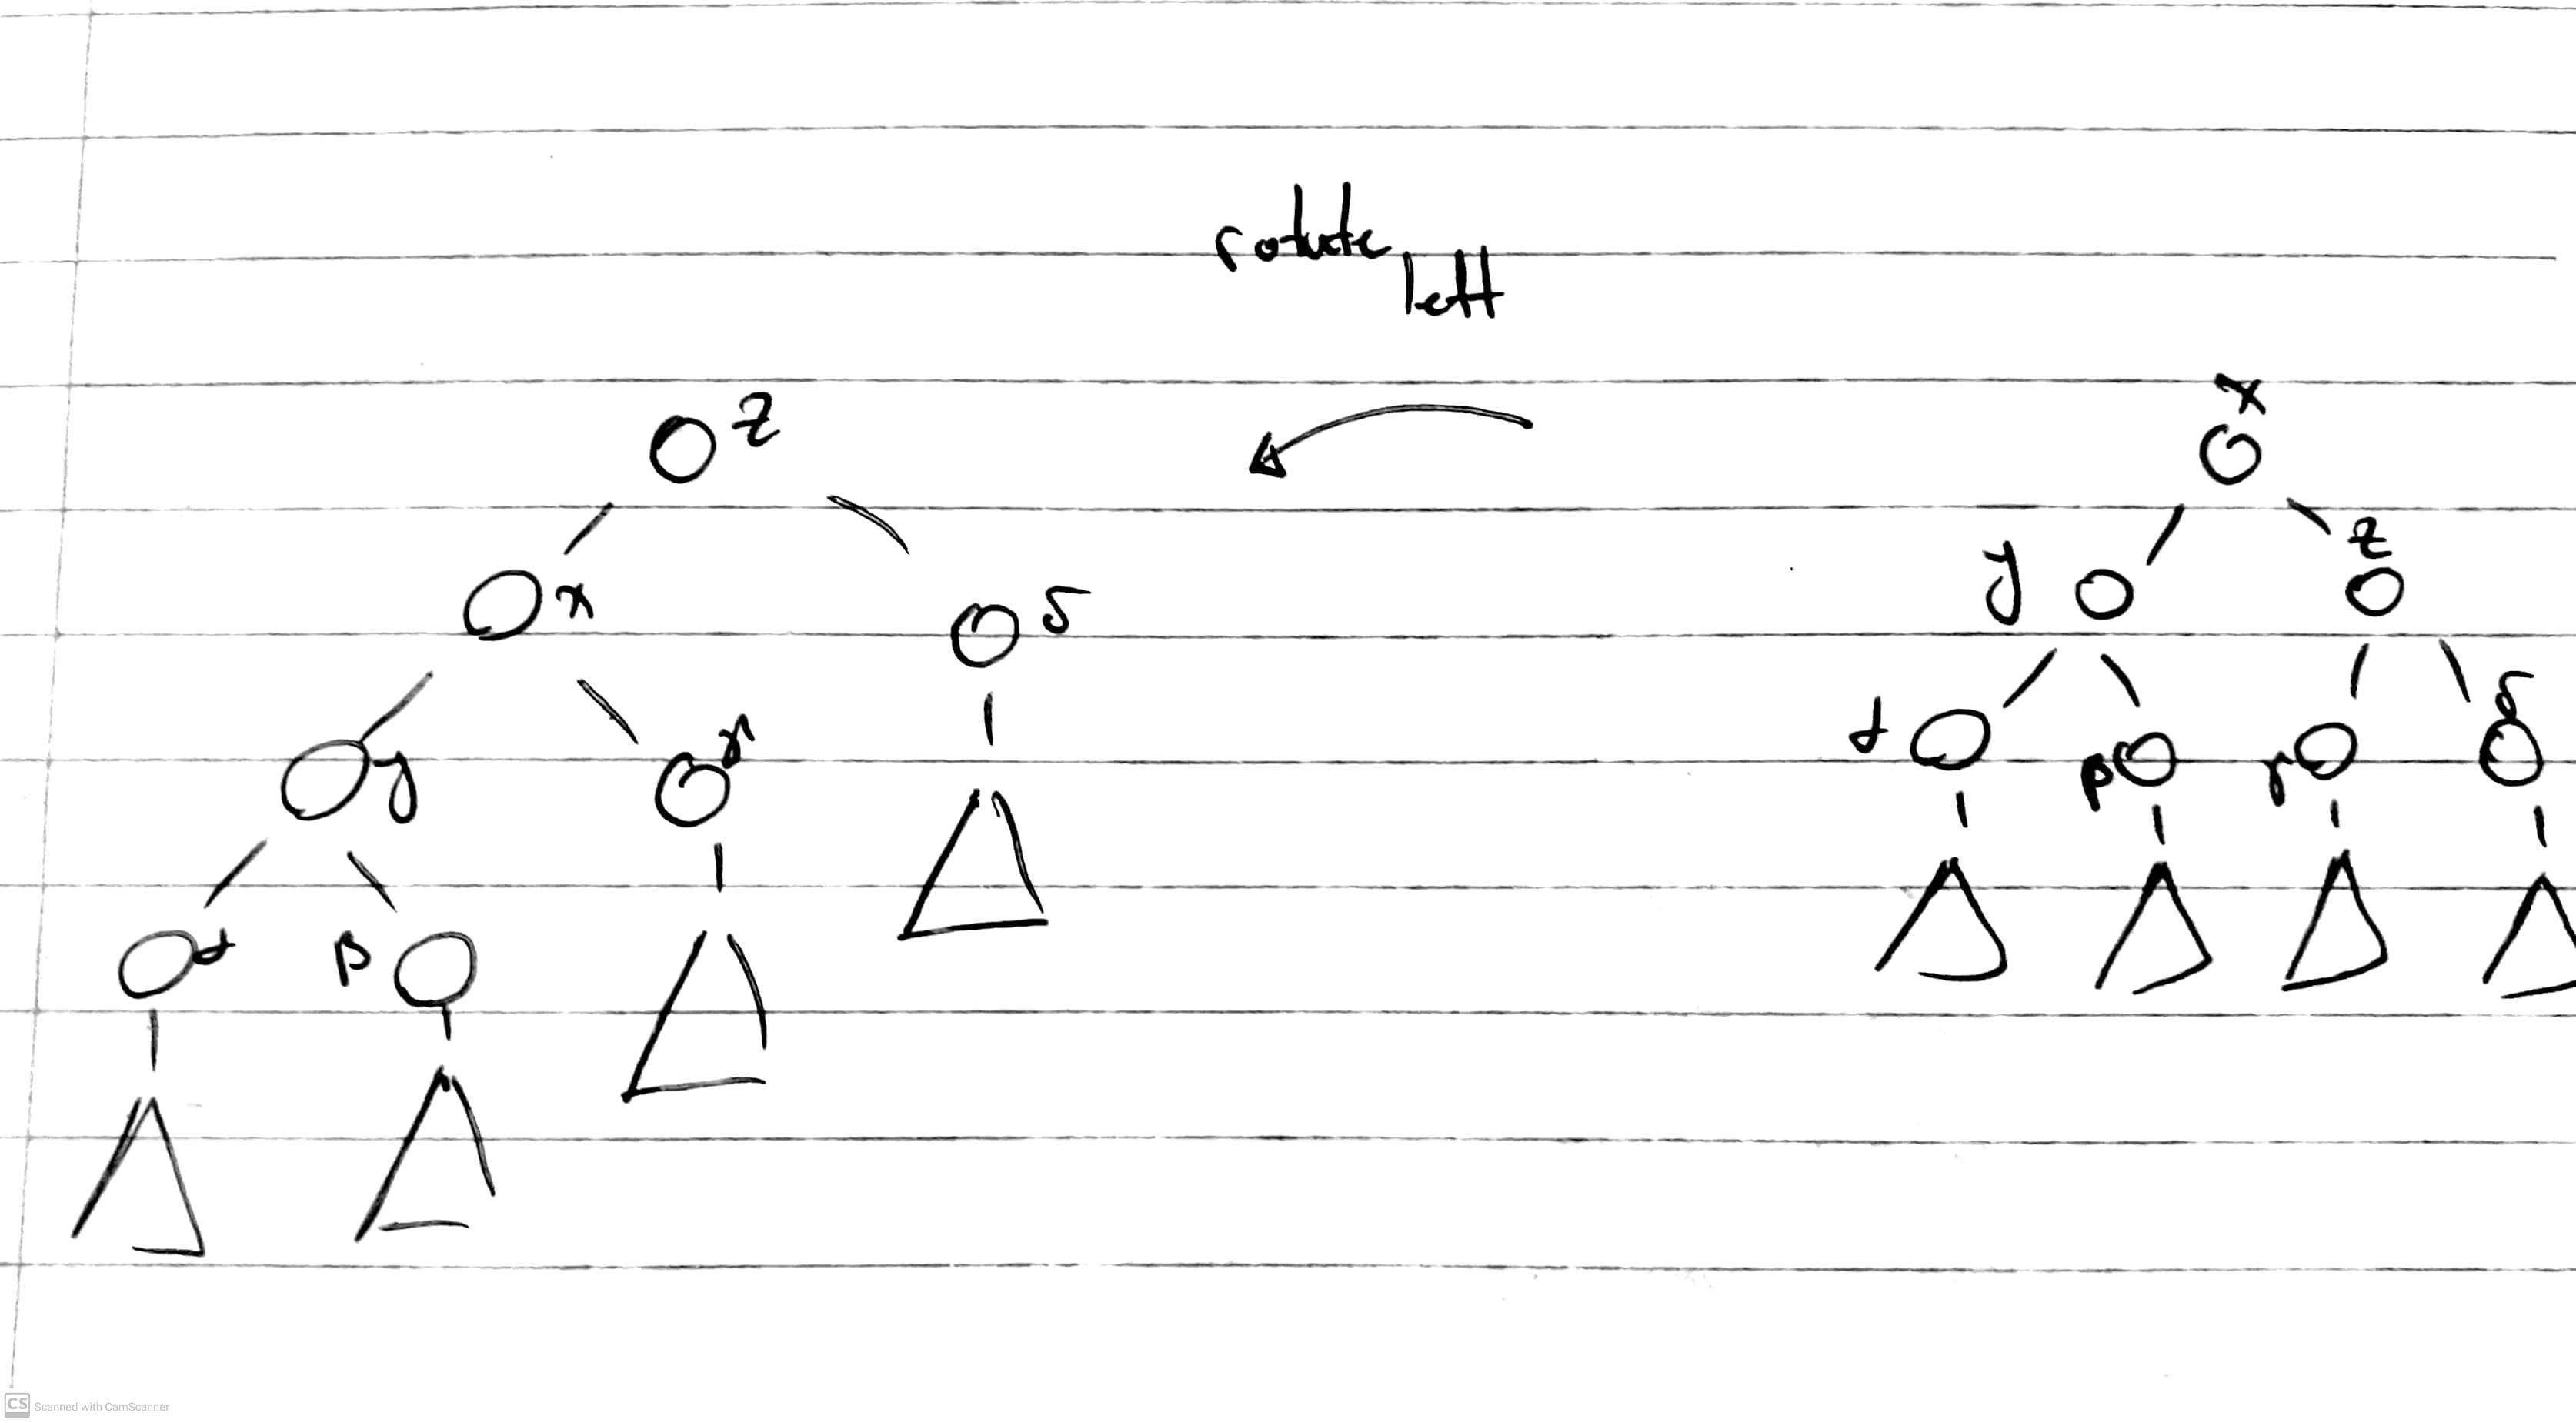
\includegraphics{tex/lectures-TA/dast_3.jpg}
    }
\end{tabular}

\paragraph{} Recall that in the last recitation, we saw how probability could help us analyze algorithms that have assumptions over the distribution of the inputs. In this recitation, we will see that using randomness can ensure that our client (who might also be our enemy) will have zero knowledge about how good or bad a particular input is. Consider the follow example:     

\paragraph{Question:} We are given \(n\) numbers \nvar{s}{n}, such \( s_i \in \left[l\right]\) for \( l > n^{15} \). Our algorithm uses the map \(f : \left[l\right] \mapsto [n] \) which defined by \(f\left(s_{i}\right) = s_{i} \left(\text{mod } n\right)\).
The algorithm returns array of \(n\) lists \(T\) where the \(j\)-th list equals \begin{equation*}
T\left[j\right] = \bigcup_{f\left(s_i\right)=j}{s_i}\end{equation*} 
Assume we are facing enemy \( E \) who wish to spoil our data base. Which input should be fed by \(E\) in order to enforce us pay a linear time for access?
Consider the following input: \begin{equation*}
\begin{split}
    s_{i} &= 1 + i\cdot n \le 1 + n^2 \Rightarrow s_{i} \in \left[l\right] \\ 
    s_1,s_2 ... s_i ... s_n & = 1 + n, \ 1 + 2n, ..., 1 + n^2 \\ 
    \Rightarrow \forall i \ \  f\left(s_i\right) &  = 1 + i\cdot n    \left(\text{mod } n\right) = 1 
\end{split}
\end{equation*}
Thus,our algorithm will maps all the strings which were sent by \(E\) into the same list.

Ok, lets try again, let \(g\) be a similar function to \(f\) defined as \( g\left(s_{i}\right) =  f\left(\left\lfloor \frac{s_i - 1}{n} \right\rfloor \right)\).
Consider the algorithm in Figure \ref{fig:my_label} which chooses the mapping function uniformly from \(\{f,g\}\). It's clear that for that algorithm the previews input is a "bad" input with probability \(\frac{1}{2}\). 
That fact raises the question, can we design a construction scheme such that all the inputs doesn't have a bias to be a bad input. \ctt{rewrite that sentence}. 

\begin{figure}[h!]
    \centering
    % \includegraphics{}
    \begin{algorithm}[H]
        \SetAlgoLined
        \KwResult{Store the values \nvar{s}{n} where \(s_i \in \mathbb{F}^{l}_{2}\) }
         \(h \leftarrow \text{ uniformly } \{ f,g \} \)
         \ \\ 
         \For{ \(i \in [n]\) }{
            \(T\left[h\left(s_i\right)\right] \leftarrow T\left[h\left(s_i\right)\right] \cup \{ s_i \} \) 
         }
         \caption{second try to construct a table}
    \end{algorithm}
    \caption{Caption}
    \label{fig:my_label}
\end{figure}

\newpage

\section{Universal Functions Family.}

\paragraph{Definition} We will say that a functions family \( \mathcal{H} = \{ h_i \}_{0}^{r} \subset \left\{ h : U \mapsto \left[m\right] \right\} \) is a \textit{universal} if for every pair \( x,y \in U \) and a function \(h\) which sampled uniformly from \(\mathcal{H} \): \begin{equation*}
    \prb{ h\left(x\right) = h\left(y\right) } \le \frac{1}{m} 
\end{equation*}  
Denote by \( C_x \) the random variable which count the length of \(h\left(x\right)\)-th list, you proved in the lecture that if \(\mathcal{H}\) is universal then the expectation of \(C_x\) is \( \mathbb{E}\left[C_x\right] \le \frac{n}{m} \). Therefore if we choose \( m = \Theta \left(n \right)\) then the expected length of each list is \( O(1) \).   

\paragraph{Construction Example.}
Denote by \(p\) a prime \( \in \mathbb{N}\) such that \(U = \mathbb{F}_{p}^{k}\). let's choose \(m=p\).
\textbf{Claim} the family: \begin{equation*}
    \mathcal{H} = \left\{h_{a}\left(x\right) = \braket{a,x}\left(\mod p\right) : a \in \mathbb{F}_{p}^{k} \right\} \text{  is universal.}
\end{equation*} 
\textbf{Proof:} let \(h \sim H\) and consider arbitrary non-equal pair \(x,y\in U\). As \(y \neq x\) there is at least one coordinate such \(x_i \neq y_i\). Assume w.l.g they are different at the \(k\)-th coordinate. And let \(z = x- y\) then the probability over \(h\) for equality is:  \begin{equation*}
\begin{split}
    \prb{h(x) =_{p} h(y)} &= \prb{\braket{a,x} =_{p} \braket{a,y}} = \prb{\braket{a,x-y} =_{p} 0 }  = \prb{\braket{a,z} =_{p} 0 } \\ &  \overset{\text{baye's rule}}{\overbrace{=}} \sum_{a_1,a_2 .... a_{k-1} \in \mathbb{F}_{p}^{k-1}}{ \prb{ \braket{a,z} =_{p} 0 | a_1,a_2 .... a_{k-1} } \prb{ a_1,a_2 .... a_{k-1} } } \\ &=    \sum_{a_1,a_2 .... a_{k-1} \in \mathbb{F}_{p}^{k-1}}{ \prb{ a_k \cdot z_k  =_{p} \overset{\text{constant} \in \mathbb{F}_{p}}{- \overbrace{a_{1}z_{1} +a_{2}z_{2} + ....+ a_{k-1}z_{k-1}}} } \prb{ a_1,a_2 .... a_{k-1} } } \\ & \overset{z_{k} \neq 0}{\overbrace{=}}     \sum_{a_1,a_2 .... a_{k-1} \in \mathbb{F}_{p}^{k-1}}{ \prb{ a_k =_{p} z_{k}^{-1} \cdot \left( \overset{\text{constant} \in \mathbb{F}_{p}}{- \overbrace{a_{1}z_{1} +a_{2}z_{2} + ....+ a_{k-1}z_{k-1}}} \right) } \prb{ a_1,a_2 .... a_{k-1} } }  \\ & \overset{\star}{\overbrace{=}}  \sum_{a_1,a_2 .... a_{k-1} \in \mathbb{F}_{p}^{k-1}}{\frac{1}{p} \cdot  \prb{ a_1,a_2 .... a_{k-1} } } = \frac{1}{p}\cdot \overset{1}{\overbrace{\sum_{a_1,a_2 .. a_{k-1} \in \mathbb{F}_{p}^{k-1}}{\cdot  \prb{ a_1,a_2 .... a_{k-1} }} }} \\ & = \frac{1}{p}
\end{split}
\end{equation*}
Where the passage in \((\star)\) steams from the fact \(p\) is prime and therefore  each \(\zeta \in \mathbb{F}_{p}\) has exactly one inverse (relative to summation action) number \(\xi \in \mathbb{F}_{p}\) such that \( \zeta + \xi =_{p} 0 \). Since the size of \( \mathbb{F}_{p}\) is \(p\) the probability that \(a_{k}\) is the inverse of right term is \(\frac{1}{|\mathbb{F}_{p}|} = \frac{1}{p} \). 

\newpage{}

\section{Perfect Hashing.}
Perfect Hashing is a construction method for ensuring that accesses, and deletion will require at most \( O(1)\) time in the worst case. The method require to know the elements from head. 
\paragraph{Perfect Hashing In Quadratic Space.} let's choose an universal hashing family \( \mathcal{H}\) such that \(4n^{2} \le m \le 8n^{2}\). The algorithm goes as follow, we will keep draw function uniformly till we will sample a function which over the input does not has any collisions.     

\begin{figure}[h!]
    \centering
    % \includegraphics{}
    \begin{algorithm}[H]
        \SetAlgoLined
        \KwResult{Store the values \nvar{s}{n} \(\in S\) }
         \(h \leftarrow \text{ uniformly } \{ \mathcal{H} \} \) \\
         Insert \nvar{s}{n} into table \(\mathbf{T}\)
         \ \\ 
         \ \\ 
         \While{ \( \exists x,y \in S\) such \(h(x) = h(y)\) }{
             \( \mathbf{T} \leftarrow \emptyset\) \\
             \(h \leftarrow \text{ uniformly } \{ \mathcal{H} \} \) \\
             Insert \nvar{s}{n} into \(\mathbf{T}\)
         }
         \ \\
         \Return \(\mathbf{T}\) 
         \caption{Hashing In Quadratic Space}
    \end{algorithm}
    \caption{Caption}
    \label{fig:my_label2}
\end{figure}
\textbf{Claim.} Let \(C_{x}\) denote the random variable which counts the collision number on the \(h(x)\) value and let \(C_{h}\) be the random variable that equal to the total number of collision, That it, \( C_{h} = \sum_{x\in S}{\frac{1}{2}C_{x}}\) . And denote by \(X\) the random variable which count the number iterations which done by the algorithm. First notice that \begin{equation*}
    \mathbb{E}\left[C_h\right]=\frac{1}{2}\mathbb{E}\left[\sum_{x\in S}{C_x}\right]\le \frac{1}{2}\sum_{x\in S}{\frac{n-1}{m}} \le \frac{1}{2}\sum_{x\in S}{\frac{n}{m}} = \frac{n^{2}}{2m} \le \frac{n^{2}}{2\cdot 4n^{2}} \le \frac{1}{2}
\end{equation*}    
So by applying the Markov inequality \( \prb{ C(h) \ge 1}\le \frac{\mathbb{E}\left[C_h\right]}{1} \le \frac{1}{2} \Rightarrow X \) is bounded by the geometric distribution with parameter \( X<X^{\prime} \sim G\left( p > \frac{1}{2}\right) \). Hence the expectation of \(X\) is bounded by \begin{equation*} \mathbb{E} \left[  X\right] \le \mathbb{E} \left[  X^{\prime}\right] = \frac{1}{p} = 2 \end{equation*}As the insertion procedure requires from us \(n\) operations, the total expectation running time is \(2\cdot n\).    
\paragraph{Perfect Hashing In Linear Space.} Based on the above method, one might try to show that the probability to sample an hash function, without collision, which maps form the keys into a linear space table is less then constant. Unfortunately, naively adjustment doesn't work here. Finding a map into a linear space table will require from us to give up over the non collision construction. Yet, It's too early to give up. 

\textbf{Claim}, for \( \{h : U \mapsto [m] \} \sim \mathcal{H}\) denote by \(n_{i}\) the random variable associate with the number of keys which mapped into the \(i\)-th cell of the table \( \mathbf{T} \) at size \(m = \Theta(n)\). Then \begin{equation*}
    \mathbb{E}\left[ \sum_{i \in [m]}{n_{i}^{2}} \right] \le 4n 
\end{equation*} 
You will be asked to prove that claim in the exercise.  
Using that result we could bound the probability to sample a function \(h\) such  \( \sum_{i \in [m]}{n_{i}^{2}} > 8n \) by: \begin{equation*}
    \prb{\sum_{i \in [m]}{n_{i}^{2}} > 8n} \le \frac{\mathbb{E}\left[ \sum_{i \in [m]}{n_{i}^{2}} \right]}{8n} \le \frac{4n}{8n} = \frac{1}{2}
\end{equation*} 
And get in similar manner to the quadratic solution that, in expectation, after constant number of rounds we will draw \(h\) which satisfy the inequality above. Then we could apply the quadratic hashing over each cell separately. The memory cost for each cell will be at order \( \Theta(n_{i}^{2})\), but since, \( \sum_{i \in [m]}{n_{i}^{2}} < 8n \) the total space cost is bounded by \begin{equation*} \sum_{i \in [m]}{ \text{cost of i`th cell}} = \sum_{i\in[m]}{\Theta(n_{i}^{2})} = \Theta(n) \end{equation*} 
\begin{figure}[h]
    \centering
    % \includegraphics{}
    \begin{algorithm}[H]
        \SetAlgoLined
        \KwResult{Store the values \nvar{s}{n} \(\in S\) }
         \(h \leftarrow \text{ uniformly } \{ \mathcal{H} \} \) \\
         Insert \nvar{s}{n} into table \(\mathbf{T}\)
         \ \\ 
         \While{ \(\sum_{x\in S}{C_{x}^{2}} > 8n\) }{
             \(\mathbf{T} \leftarrow \emptyset\) \\
             \(h \leftarrow \text{ uniformly } \{ \mathcal{H} \} \) \\
             Insert \nvar{s}{n} into \(\mathbf{T}\)
         }
         \ \\
         \For{ \(i \in [m]\) }{
         \(\mathbf{T}\left[i\right] \leftarrow\) Hashing In Quadratic Space \( \mathbf{T}[i] \)
         }
         \Return \(\mathbf{T}\) 
         \caption{Hashing In Linear Space}
    \end{algorithm}
    \caption{Caption}
    \label{fig:my_label2}
\end{figure}

\newpage{}

\section{Quick Sort.}

Recall the quick sort algorithm. Let \(X^{n}_{ij}\) be the indicator for the event there was a comparison between \(A^{\star}_{i}\) and \(A^{\star}_{j}\) where \(A^{\star}\) is the sorted array at length \(n\). 

\textbf{Claim.} \( \mathbb{E}[X^{n}_{ij}]\) doesn't deepened on \(n\) and equals to \( \frac{2}{j-i + 2} \). \textbf{Proof:} by induction over \(n\) in the base case \(n = j-i+2\) and hence every choice for the pivot in the range \( (i,j) \) will the seprate values \(A^{\star}_{i}\) and \(A^{\star}_{j}\) into diffident arrays. Therefore the only cases in which the comparison occur are the pair where one of those values is chosen as pivot. The probability for that happened is \begin{equation*} \frac{2}{n} = \frac{2}{j-i +2} \Rightarrow  \mathbb{E}[X^{j-i+2}_{ij}] = \frac{2}{j-i +2} \end{equation*} Assume the correction of the Claim for every \(j-i+2 < n^\prime < n\) and by the baye's rule we get: 
\begin{equation*}
\begin{split}    \mathbb{E}[X^{n}_{ij}] &= 1\cdot\prb{X^{n}_{ij}} = \sum_{p\in [n]}{1\cdot\prb{X^{n}_{ij}| p}\prb{p}} \\ &= \sum_{p^{\star} \in \{i,j\} \}}{1\cdot\prb{X^{n}_{ij}| p}\prb{p}} +  \overset{0}{\overbrace{\sum_{p^{\star} \in (i,j) }{1\cdot\prb{X^{n}_{ij}| p}\prb{p}}}} \\ & + \sum_{p^{\star} \in n/[i,j] }{1\cdot\prb{X^{n}_{ij}| p}\prb{p}} = \frac{2}{n} + \left(1 - \frac{j-i+2}{n} \right)\frac{2}{j-i+2} \\ &= \frac{2}{j-i+2}
    \end{split}
\end{equation*}

\begin{figure}[h!]
    \centering
    % \includegraphics{}
    \begin{algorithm}[H]
        \SetAlgoLined
        \KwResult{Sort the values \nvar{A}{n}  }
        
        \If { \(n = 1\)}{
            \Return \(A_{1}\)
        } 
        
         \(p \leftarrow \text{ uniformly } \left[n\right] \) \\
         \( S_{l} , S_{r} \leftarrow  \emptyset, \emptyset\)
         \ \\ 
        \For{ \(i \in [n]\) }{
            \If{ \( A_{i} \le A_{p} \)}{
                \(S_{l} \leftarrow S_{l} \cup \{A_{i}\}\)
            }
            \Else{
                \(S_{r} \leftarrow S_{r} \cup \{A_{i}\}\)
            }
        }
        Quick Sort \( ( S_{l} ) \) \\
        Quick Sort \( ( S_{r} ) \)\\
        \Return \( [ S_{l}, A_{p}, S_{r} ]\)  
         \caption{Quick Sort}
    \end{algorithm}
    \caption{Caption}
    \label{fig:my_label2}
\end{figure}

So in total the excepted running time is 
\begin{equation*}
    \begin{split}
        \mathbb{E}\left[\text{comparisons}\right] &= \sum_{i\in n}{\sum_{j \in [i +1,n]}{\mathbb{E}[X_{ij}]}} = \sum_{i\in n}{\sum_{j \in [i +1,n]}{\frac{2}{j-i+2}}} \\ & \le \sum_{i\in n} \int_{i+1}^{n}{\frac{2}{j-i+2 }dj} = \Theta\left(n \log n\right)
    \end{split}
\end{equation*}


% \printbibliography 
\end{document}


